%\td{https://en.wikipedia.org/wiki/Thesis}
\ds{what is it? What is it used for? How does it work? What different kinds are there? }
\ds{what? how? why?}
This chapter can be broken down into three sections. 
The first section tries to shine light on the evolution of PV and give some background on \gls{cigs}.
The middle section reads about material-scientific methods which were used during the practical part of this work. 
The last and third part focuses on the information technological, algorithmic and analytics methods used to optimize and predict material properties. 

\subsection{Photovoltaics}
%%%%%%%%%%%%%%%%%%%%%%%%%%%%%%%%%%%%%%%%%%%%%%%%%%%%%%%%%%%%%%%%%%%%%%%%%%%%%%%%%%%%%%%%%
%%%%%%%%%%%%%%%%%%%%%%%%%%%%%%%%%%%%%%%%%%%%%%%%%%%%%%%%%%%%%%%%%%%%%%%%%%%%%%%%%%%%%%%%%
\subsubsection{Problems of current energy supply}
The world wide energy consumption has more than doubled between 1970 and 2015\cite{BP2017} 
and according to recent studies both fossil\cite{BGR2017} and uranium sources\cite{Uran2006} 
will be exhausted within the next 100 years. 
Even though this time period is not exact and highly dependent on detection methods of resources, 
this number is rather small and brings us in zugzwang to develop sustainable energy sources. 
One viable options is \gls{pv}.

%%%%%%%%%%%%%%%%%%%%%%%%%%%%%%%%%%%%%%%%%%%%%%%%%%%%%%%%%%%%%%%%%%%%%%%%%%%%%%%%%%%%%%%%%%%%%
\subsubsection{History of Photovoltaics}
The photoelectric effect was first described in 1839 by french scientist Alexandre 
Edmond Becquerel, the father of Henri Becquerel\cite{becquerel1839memoire} (the person after whom the unit is named).
Another relevant piece of the \gls{pv} jigsaw was discovered 
with the discovery of photo conductivity of selenium
by British engineer Willouhgby Smith\cite{Smith1873Selenium}.
In 1876 William Adams and Richard Day\cite{Adams1876Selenium} showed that 
the energy of light can be directly converted into electrical energy by a bar of 
selenium with attached platinum electrodes.
And finally, in 1905 Einstein described the physical background of the photoelectric 
effect with his light quantum theory\cite{einstein1905erzeugung}.
In the 1950s the first solar cells (with efficiencies under 10 percent) were used in niche applications such as space flight. 
Eventually, the interest in photovoltaic and other alternative energy sources 
rose - fuelled by the oil crisis in 1973 - 
and the development of photovoltaic for the consumer market was boosted. 
This development lead to a drop in 
average price for \gls{pv} module from \$ 100 per watt in 1975 to \$ 4 per watt in 2007\cite{pagliaro2008flexible}.

%%%%%%%%%%%%%%%%%%%%%%%%%%%%%%%%%%%%%%%%%%%%%%%%%%%%%%%%%%%%%%%%%%%%%%%%%%%%%%%%%%%%%%%%%%%%%
\subsubsection{Crystalline Silicon Photovoltaics}
\td{aka PV basics}
The proecess of conversion of photons into voltaic energy can be broken down into two essential steps (both in silicon based \gls{pv} or in plants): 
the creation of an electron hole pair and then their separation by the structure of the device. 
This means that \gls{pv} cells are basically diodes, which have a low resistance in one direction and a high resistance in the other direction.
\td{stop}
The first marketable \gls{pv} were crystalline silicon photovoltaic modules which still have the biggest market share in the \gls{pv} segment including polycrystalline and monocrystalline silicon.
\td{what is it? What is it used for? How does it work? What different kinds are there? }
\cite{markvart2013principles}
\td{CIGS has higher absorption coefficient because of direct band gap in contrast to crystalline silicon which has an indirect band gap and therefore less absorption probability.}

%%%%%%%%%%%%%%%%%%%%%%%%%%%%%%%%%%%%%%%%%%%%%%%%%%%%%%%%%%%%%%%%%%%%%%%%%%%%%%%%%%%%%%%%%%%%%
\subsubsection{CIGS}
CIGS ($\text{CuIn}_\text{x}\text{Ga}_{\text{(1-x)}}\text{Se}_2$) is of the chalcopyrite group (tetragonal crystal system) and can be used as thin film \gls{pv}. 
Just like CdTe, GaAs and amorphous silicon CIGS have much higher absorption coefficients 
(lower penetration depth) of visible light than crystalline silicon (see table \ref{tab:cigs:alpha}). 
These thin film \gls{pv}s not only use less material, but also can be used in flexible applications. 

\begin{table}[htb]
	\small
    \center
    \begin{tabular}{cccccc}
        \hline
        \hline
		Material&   Type&    Band Gap [\ev{}]&    Wavelength [\nm{}]&    Absorption coef. $\alpha$ [\pcm{}]    &Penetration Depth [\um{}]\\
        \hline
		c-Si&   indirect&   1.12&   600&    \num{4000}&    2.5\\
		c-Si&   indirect&   1.12&   1000&    \num{64}&    150\\
		c-Si&   indirect&   1.12&   1100&    \num{3.5}&    290\\
		a-Si&   direct&      1.7&    600&    \num{40000}&  0.25\\
		CdTe&   direct&      1.45&    600&    \num{37000}&  0.3\\
		GaAs&   direct&      1.42&    600&    \num{40000}&  0.2\\
        \hline
        \hline
    \end{tabular}
	\caption{data from \cite{mertens2015photovoltaik}}
	\label{tab:cigs:alpha}
\end{table}

Amazingly, the band gap of CIGS can be varied between 1eV and 1.7eV by varying the indium gallium ratio.
This is a result of the large difference of band gaps of \ch{CuInSe2} and \ch{CuGaSe2} (see table \ref{tab:cigs}). 

\td{Bild: electrode + n-ZnO, [2.42eV] n-CdS 40nm, [1.15eV] p-CIGS 1.5um, Molybden 0.5 um, glass substrate, borrow book (Recreated based on\cite{mertens2015photovoltaik}) or (Image source:\cite{mertens2015photovoltaik})}
\begin{figure}
	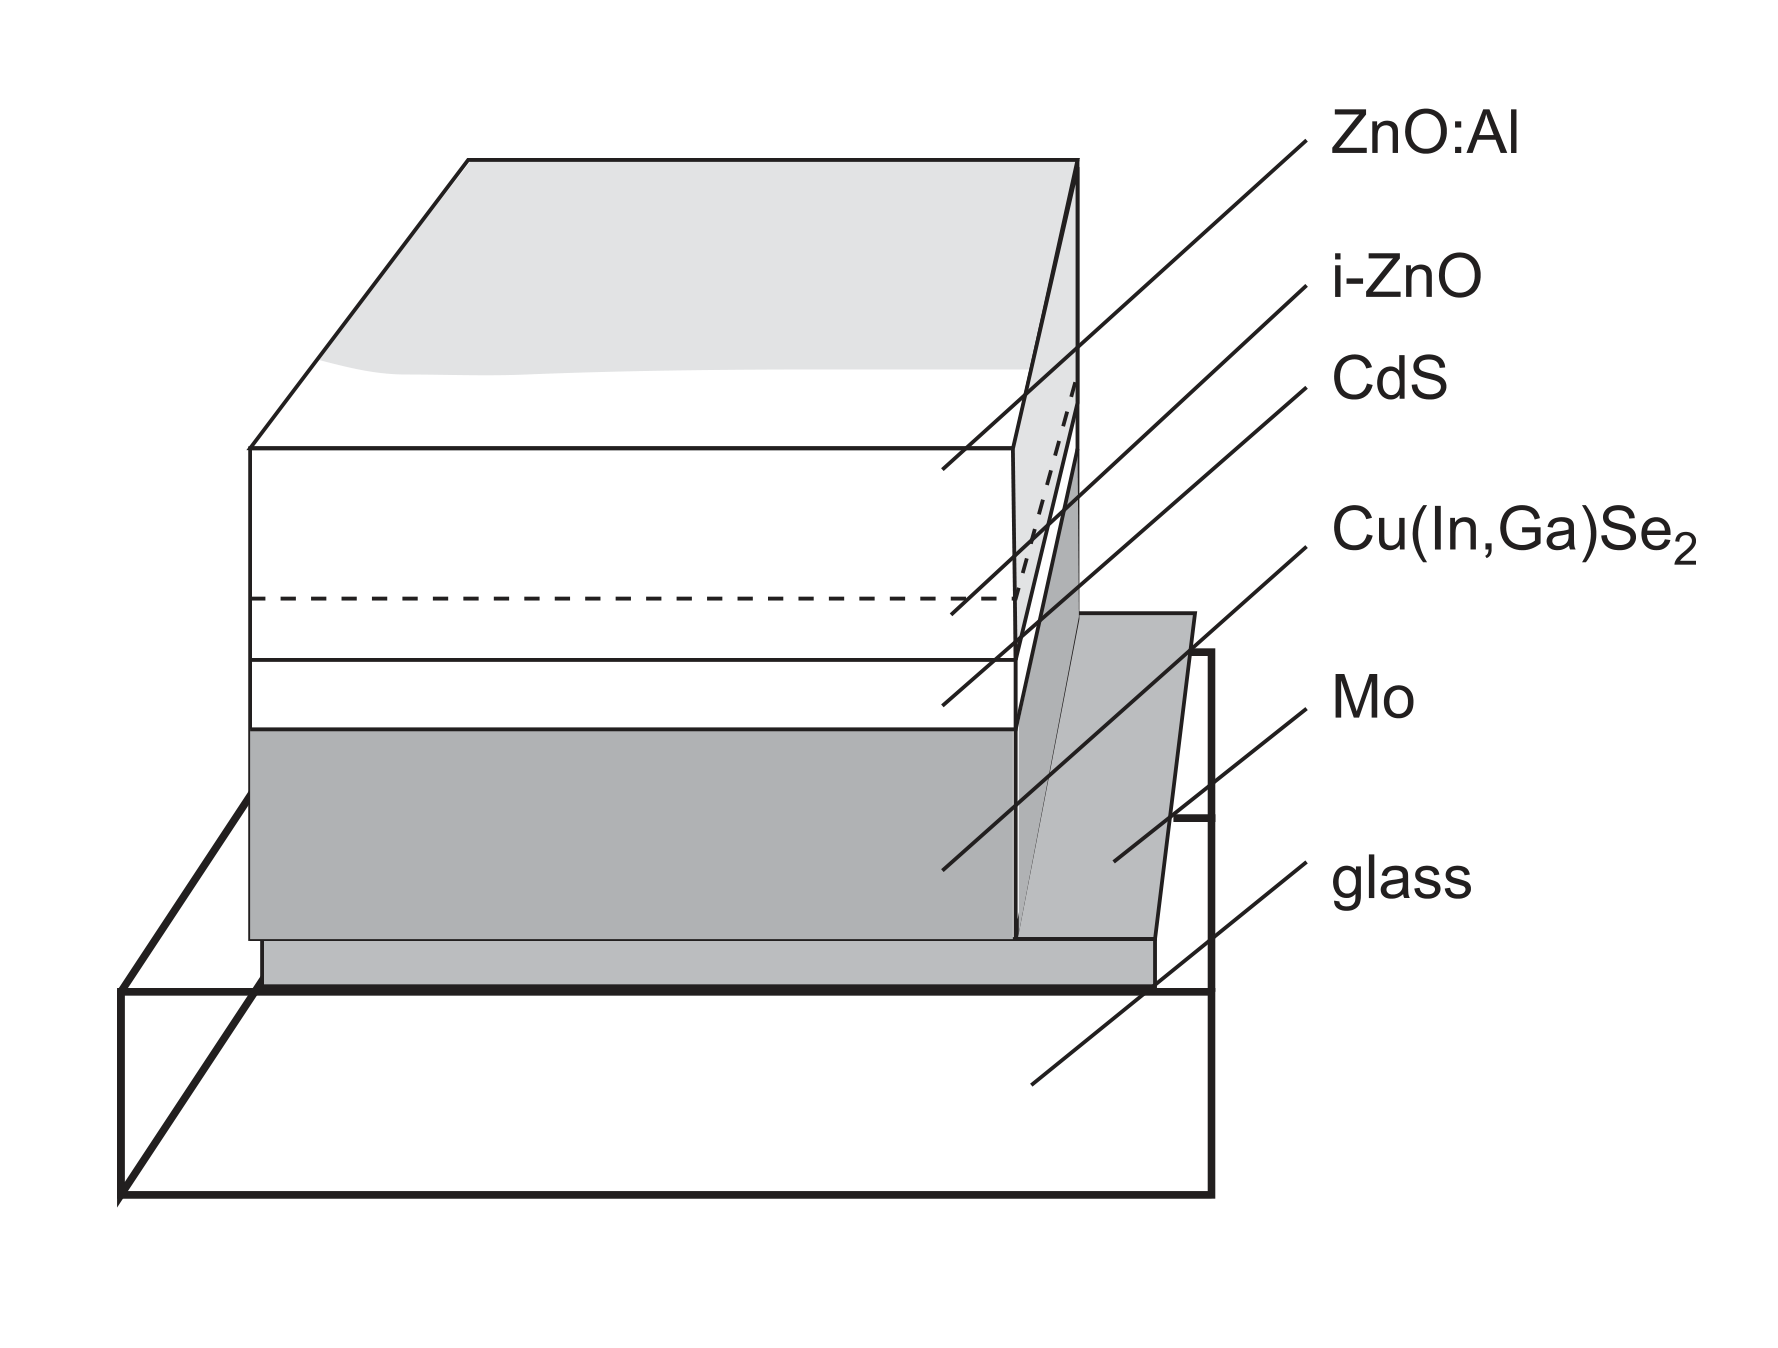
\includegraphics[width=\textwidth]{./Pics/cigs.png}
\end{figure}

The standard substrate is glass 
because of it's high thermal stability, resistance and hardness. 
A flexible substrate is needed for a flexible module, though. 
Plastics have a very low melting points and metals are conducting, but can be coated with a non conducting material such as \gls{zro}.
\begin{table}[htb]
    \center
    \begin{tabular}{cccc}
        \hline\hline
        Empirical Formula&    Name&   Band Gap&    Abbreviation\\
        \hline
		\ch{CuInSe2}&       copper indium di selenide&  1&  CISe\\
		\ch{CuInS2}&        copper indium di sulfide&  1.5&  CIS\\
		\ch{CuGaSe2}&       copper gallium di selenide&  1.7&  CIGSe\\
		\ch{CuGaS2}&        copper gallium di sulfide&  1.55&  CIGS\\
        \hline\hline
    \end{tabular}
	\caption{band gaps of different chalcopyrites}
	\label{tab:cigs}
\end{table}

%%%%%%%%%%%%%%%%%%%%%%%%%%%%%%%%%%%%%%%%%%%%%%%%%%%%%%%%%%%%%%%%%%%%%%%%%%%%%%%%%%%%%%%%%%%%%
%%%%%%%%%%%%%%%%%%%%%%%%%%%%%%%%%%%%%%%%%%%%%%%%%%%%%%%%%%%%%%%%%%%%%%%%%%%%%%%%%%%%%%%%%%%%%
\subsection{Materials and Their Analysis}
\subsubsection{Zirconium oxide}
Zirconium oxide \gls{zro} is a ceramic with a band gap of 5-7 eV and dielectric constant of 15-22 at room temperature\cite{Anwar2017}. 
This makes it attractive as an insulator for semiconductor and \gls{pv} industry. 
It is monoclinic below 1050 °C, tetragonal between 1170 °C and 2370 °C, and cubic above 2370 °C\cite{Nielsen2005}.
The cubic phase can be stabilzed down to room temperature by the addition of magnesia (\ch{MgO}), calcia (\ch{CaO}) or yttria (\ch{Y2O3}) which avoids mechanical failing due to shrinkage 
when cooling and undergoing phase transistion\cite{Nielsen2005}.
It is very resistant to acids (except \ch{HF} and hot \gls{h2so4}) and alkalis\cite{Nielsen2005}.
Hydrous Zirconium Oxide (\ch{Zr(OH)8 * 16 H2O}) gel can be produced by neutral hydrolysis of sodium zirconate (\ch{NaZrO3}). 
"Zirconium alkoxides hyrdolize quite easily, [providing] a route to high purity, high-surface-area zirconium oxide"\cite{Nielsen2005}.

%%%%%%%%%%%%%%%%%%%%%%%%%%%%%%%%%%%%%%%%%%%%%%%%%%%%%%%%%%%%%%%%%%%%%%%%%%%%%%%%%%%%%%%%%%%
\subsubsection{Sol-Gel and Doctor Blading}
\td{what is it? What is it used for? How does it work? What different kinds are there? }
One of the advantages of sol-gel process is that it can be used in roll-to-roll procedures.

%%%%%%%%%%%%%%%%%%%%%%%%%%%%%%%%%%%%%%%%%%%%%%%%%%%%%%%%%%%%%%%%%%%%%%%%%%%%%%%%%%%%%%%%%%%
\subsubsection{Sputtering}
%SPUTTERING FREEWRITING: 
%what is sputtering? \\
Sputtering is the processes of highly energetic ions hitting a surface and atoms or molecules being expelled. 
This is called a physical vapor deposition (PVD) technique. 
PVD can be divided into activation by thermal energy and activation by energetic particle bombardment. 
Sputtering is of the latter, which 
is advantageous if substrates can't withstand high temperatures.
%\td{what can it be used for?}\\
Sputtering evolved from being a curious experiment in the middle of the 20th century to having various applications in research and engineering.
Use cases vary from thin films depositions for \gls{pv}, for electrical circuits or for storage media such as CDs and DVDs 
over sputter cleaning and etching to analysis.
Advantages of 
sputtered thin films include good adhesion to the substrate and good step coverage\cite{Swann1988}.

%\td{how does it work?}\\
A high voltage is applied to 
two parallel electrodes with low pressure gas in between. 
The target acts as cathode and the substrate (holder) as anode (see \td{fig}).
%the target which acts as a cathode with the substrate as anode in a parallel geometry (see \td{fig}).
The cathode, then, emits electrons which collide with a gas particles (mostly argon because of it's inert properties and potential to transfer more kinetic than lighter noble gases). 
Some gas particles may get ionized by the collision and the gas cations are accelerated to the cathode. 
If a cation has enough energy it will bump off one or more atoms or molecules from the surface. 
This happens by a cascade of momentum transfers, which can reach the surface again (see fig \td{cp sigmund69}). 
If a surface particle obtains momentum pointing away from the bulk and its kinetic energy is higher than the binding energy, the particle is sputtered. 
This sputtered particle travels unaffected by the electrical field perpendicular to the surface towards the substrate and condenses with other particles to form a layer.
The pressure should be small, such that the sputtered particle has a long \gls{mfp}, but on the other hand 
a minimum pressure is needed to keep the plasma "alive". 
Usual pressures are around \SI{1}{\Pa} (\num{e-2}\SI{}{\milli\bar}) or lower\cite{Swann1988}.

A magnetron can be placed behind the cathode (target) in order to trap ejected electrons close to the source. 
This prevents high energy electrons from reaching the target and undoing the deposited layer and this also increases the probability of an electron colliding with an argon atom and ionizing it, increasing the yield.

When oxygen or nitrogen are added to the  gas this is called reactive sputtering.
Sputtered atoms will react with the gas and result in oxide or nitrides layers, respectively.
The stoichiometry of the resulting layer can be regulated by gas ratios, but too much reactive gas can lead to target poisoning. 
Meaning the target begin covered by an insulating layers which can lead to defects in the growing film\cite{Kelly2000}. 

The limitation of only being able to use conducting materials as targets can be circumvented by using a radio frequency electrical field. 
This prevents a charge building up on the target. %\td{why is a charge?}
Although RF sputtering is more versatile, DC sputtering is more common because of it's simpler system and economical reasons.
%\td{sputtered particles are neutral and not influenced by the electrical field}

%%%%%%%%%%%%%%%%%%%%%%%%%%%%%%%%%%%%%%%%%%%%%%%%%%%%%%%%%%%%%%%%%%%%%%%%%%%%%%%%%%%%%%%%%
\subsubsection{Scanning electron Microscopy}
The history of \gls{sem} can be traced back to 1843 when Scottish clockmaker Alexander Bain filed a patent for dissecting an image by scanning. A detailed history of \gls{sem} can be read in a open-to-read paper by McMullan from 1995\cite{McMullan1995}. 
\Gls{sem} is a microscopical technique which allows visualisation of surfaces with features in the nano meter regime. 
While optical microscopes use visible light and optical lenses, \gls{sem} uses accelerated electron beams and electrostatic and electromagnetic lenses.
This allows the generation of much more detailed images due to the shorter wavelengths of electrons compared to light\cite{Kaliva2020}.
The electron beam produces X-rays, elastically backscattered (primary) electrons, inelastic (secondary) electrons and Auger electrons. 
Secondary electrons carry information to conclude morphology and topology of the sample while X-rays can be used to identify the elements. 
Electrons originate from either \gls{feg}, where are strong electrical field rips electrons from the bulk, or from thermionic guns where the filament (tungsten W or \ch{LaB6} (brighter and longer lasting but more expensive)) is heated until electrons are emitted. 
Electrons are then accelerated by a voltage of 2 to 40 kV and bundled into narrow beams\cite{Vernon2000} by lenses.
A high \gls{mfp} is needed for electrons to travel from the source to the sample (and to the detector). 
Thus, a very low pressure is in the inside. 
In this work \gls{sem} was used as a preliminary way of checking the surface condition. 


%%%%%%%%%%%%%%%%%%%%%%%%%%%%%%%%%%%%%%%%%%%%%%%%%%%%%%%%%%%%%%%%%%%%%%%%%%%%%%%%%%%%%%%%%
\subsubsection{Infrared Absorption and Spectroscopy}
%%% WHAT? 
\Gls{ir} spectroscopy is a molecular spectroscopic method using interactions of \gls{ir} light (wavelengths $\lambda$ of \num{e-3} to \num{e-6}\m{}
or wave numbers $\bar{\nu}$ of 500 to \pcm{4000} ) with molecules. \cite{Schwedt2008}
In general, light is described as periodic \gls{em} wave 
which - in vacuum - moves with the speed of light ($c = \mps{299792458}$).
The relation of energy~$E$ of a photon, its frequency~$\nu$, wavelength~$\lambda$ and wave number~$\bar{\nu}$ are as follows:
\begin{align*}
	E &= h \cdot \nu \\
	\nu &= c/ \lambda \\
	\bar{\nu} &= 1/\lambda,
\end{align*}
where $h$ is the Planck's constant.
%In words: shorter wavelength (higher frequency) photons are more energetic.
In practice the spectrum of \gls{em} waves is sectioned into different ranges (\td{see figure?});
from high to low energy: X-ray, \gls{uv}, \gls{vis}, (near, middle and far) \gls{ir}, microwaves and radio waves. 
\td{with number?}
X-rays interact with core electrons, \gls{uv}\gls{vis} with valence electrons, \gls{ir} with molecular vibrations, microwaves with molecular rotations and radio with electron and nuclear spins. 
%Molecular vibrations can be separated in valence and deformation vibrations.
%
A molecule has $F=3N$ ($N$ number of atoms) degrees of freedom, including translational $F_T=3$ and rotational $F_R=3$ (2 for linear molecules) movements. 
%
The number of vibrations can therefore calculated as 
\begin{align*}
	F_V &= 3N - F_T - F_R = 3N - 6 \\
	F_V &= 3N - F_T - F_R = 3N - 5 \textrm{ (for linear molecules)}.
\end{align*}
Vibrations are classified in valence vibrations (change of bond length) and deformation (change of bond angle) vibrations\cite{Melker2006}. 
Only vibrations that change the dipole moment of the molecule are \gls{ir} active. 

%\td{describe simple IR with monochromator}

\paragraph{(Fourier Transform) Infrared spectrometer}
 A ceramic material (Nernst glower) is heated to around \oc{1600} as light source. 
 In the two-beam-spectrometer the light is split, sent through the sample and a reference and one of the two beams is alternately sent through a monochromator to a detector (\td{thermocouple}). 
%
In the \gls{ft}\gls{ir} spectrometer the beam is sent through the sample, split and 
reflected from a static and from a moving mirror, recombined and detected by a photo 
multiplier (a device which transforms photons into electrical signals). 
How the two beams will interfere upon recombination depends on the optical path difference (also called retardation) of the two light beams\cite{Schwedt2008}.
In a \gls{ft}\gls{ir} spectrometer the reference has to be measured before the sample.
%
When the refractive index of two layers differ, \gls{ir} can be used to measure the thickness\cite{Dumin1967} of optical less dense material.

%\td{Frank-Condon rules, spin verbot and symmetrie verbot are ausschlaggebend für the resulting spectrum. }
%differences to \gls{uv}\gls{vis}: transmission instead of absorbance, higher energy left instead right in plot, base line on top instead of bottom.

\td{QUESTIONS: 
	how does detector work? two different for UVVis and MIR
	IR around page 45;
The absorbance intensity is dependent on wave length and molecule structure. 
Absorbance per din 1349: $A(\lambda) = \log{\frac{\phi_{in}}{\phi_{ex}}}$ and transmission $\tau =T=D= \phi_{ex}/\phi_{in}$
}


%%%%%%%%%%%%%%%%%%%%%%%%%%%%%%%%%%%%%%%%%%%%%%%%%%%%%%%%%%%%%%%%%%%%%%%%%%%%%%%%%%%%%%%%%
\subsubsection{X-Ray Diffraction}
%\url{https://link.springer.com/content/pdf/10.1186/2228-5326-3-8.pdf}
\gls{xrd} is used to study the crystalline structure of materials.
Since X-rays wavelengths (\num{0.2} to \nm{10}) are comparable to the interatomic spacing of crystalline solids the beams get reflected and contain information about the structure\cite{Kaliva2020}.
Each crystalline material has a discreet atomic structure, which upon irradiation with 
X-rays causes constructive and destructive interference according to Bragg's law and generates unique diffraction patterns. 
\Gls{xrd} diffraction plots of crystalline materials feature distinct peaks, whereas amorphous materials exhibit a broad curve with a maximum extending over several degrees (2$\theta$).

%\url{https://chem.libretexts.org/Courses/Franklin_and_Marshall_College/Introduction_to_Materials_Characterization__CHM_412_Collaborative_Text/Diffraction_Techniques/X-ray_diffraction_(XRD)_basics_and_application}\\


%%%%%%%%%%%%%%%%%%%%%%%%%%%%%%%%%%%%%%%%%%%%%%%%%%%%%%%%%%%%%%%%%%%%%%%%%%%%%%%%%%%%%%%%%
%%%%%%%%%%%%%%%%%%%%%%%%%%%%%%%%%%%%%%%%%%%%%%%%%%%%%%%%%%%%%%%%%%%%%%%%%%%%%%%%%%%%%%%%%
%%%%%%%%%%%%%%%%%%%%%%%%%%%%%%%%%%%%%%%%%%%%%%%%%%%%%%%%%%%%%%%%%%%%%%%%%%%%%%%%%%%%%%%%%
\subsection{Machine Learning and Statistics}
%%%%%%%%%%%%%%%%%%%%%%%%%%%%%%%%%%%%%%%%%%%%%%%%%%%%%%%%%%%%%%%%%%%%%%%%%%%%%%%%%%%%%%%%%
\subsubsection{Artificial Inteligence and Machine Learning}

The history of \gls{ai} goes back to the middle of the \nth{20} century. 
Researchers from the emerging field came together at the Dartmouth conference and the term "\gls{ai}" was coined\cite{McCarthy1955}. 
For a more in depth dive into the history of AI consult the beautifully written review\cite{Apter1982} of McCorduck's 1982 book "Machines Who Think"\cite{McCorduck1982}, which focuses also on the great minds behind advances of \gls{ai}.
Pioneers like Alan Turing thought a lot about how to define, test and implement \gls{ai}\cite{Howard2019}. 
One example how to measure \gls{ai} is to let it play chess against a human\cite{Silver2017} 
(in 1997 a chess computer called Deep Blue won against the World Chess Champion Garry Kasparov for the first time\cite{Feng1999}).
Another test ingenioused by Alan Turing, is that a human communicates with an unknown entity (in written form) and must judge if they are dealing with a machine or a human being. 
It is easy for humans to come up with question to detect an AI, 
but when reading AI written articles\cite{gpt2020}, it's easy to see this test being passed in the near future. 

But fear not, that doesn't mean that computers are sentient or more intelligent than humans\cite{searle1980,searle1999married} and certainly not that research is over. 
AI is still a young field, which is strongly growing and is gaining ubiquitous status. 
It is slowly creeping into every aspect of modern human life just like electricity around one hundred years ago. 
%Now, we can't - it's hard to - imagine to live without electricity. 
Realms in which AI is gaining traction are: 
%
playing board games (and beating humans)\cite{Silver2017,Feng1999,Campbell2002}, 
image recognition (in medicine)\cite{Li2020,Deo2015,Topol2019,Fujiyoshi2019}, 
in chemistry\cite{Westermayr2019,goh2017chemception,jha2018elemnet}, 
cyber security\cite{Sarker2021},
facial recognition (to prevent theft of toilet paper \cite{Andrews2017}),
financial sector (as robo-advisors)\cite{Littman2021},
natural language processing (NLP)\cite{Koroteev2021,Liu2021gpt,Parviainen2021} (which can also create pictures through scalable vector graphics (SVG) and code)
and even creative tasks like 
creating non existing faces\cite{Mansourifar2020}, 
create artwork (DALL-E 2)\cite{Marcus2022} or 
making video games\cite{Guzdial2016}.
%
It is nearly hard to find a field where \gls{ai} isn't used in some way. 
This steady incorporation of \gls{ai} leads to the so called \gls{ai} effect\cite{McCorduck1982,ai100}: 
certain fields get incorporated into \gls{ai} research and practice and after some time of general use are no more considered \gls{ai} (e.g. spam filter or web searches).
Google CEO Sundar Pichai even goes as far and said: 
"AI is one of the most important things humanity is working on. It is more profound than [...] electricity or fire"\cite{Hassan2020}

%
%%%%%%%%%%%%%%%%%%%%%%%%%%%%%%%%%%%%%%%%%%%%%%%%%%%%%%%%%%%%%%%%%%%%%%%%%%%%%%%%%%%%%%%%%
\subsubsection{Machine Learning Methods}
There is a platitude of different machine learning methods: 
they can be divided into supervised (training set is labeled) and unsupervised (exploratory).  
An orthogonal division can be made by regression (continuous) versus classification (discrete). 
Independent from these $2\times2$ categories there are multiple ways to let machines learn from data.
\Gls{nn} (one of the most popular architectures for big data\cite{Chiroma2019}) are loosely modeled after the brain\cite{bishop1994neural}.
%
Artificial neurons (also called nodes), which are arranged in layers, 
are connected to each of the neurons of previous and next layers
and the weights (parameters of intensity), with which the data is routed from one neuron to another, 
are optimised during training. 
%
Convolutional-layer \gls{nn} excel in picture recognition\cite{Lecun1995conv} and in quantum mechanics too\cite{westermayr2020combining}.
Other common \td{architectures} are linear regression, kernel ridge regression, support vector regression.
There are also lesser know algorithms like 
evolutionary algorithms (e.g. \gls{ga} and \gls{pso}).
%
One advantage of evolutionary algorithms is that they start with a small data set
and periodically request new data in order to solve the problem iteratively.

A genetic algorithm (GA) is a search algorithm that uses principles of natural selection and genetics to optimize a search space. A GA starts with a population of randomly generated solutions, or chromosomes, and then proceeds to breed them together to create new solutions. The new solutions are then tested for fitness, and the best solutions are selected to create the next generation of chromosomes. This process is repeated until a satisfactory solution is found.\footnote{This paragraph was written by GPT\cite{Liu2021gpt} providing the input "Introduction to genetic algorithms: "}

\iffalse
\Gls{ga} uses a starting population of size $p$ ($p \in$ \td{N$^+$}) where each experiment (or data point) 
is represented by a fixed size genome of 0's and 1's in most cases. 
Each individual is then given a fitness value. 
New genomes are added and discarded from the population using 
selection, mutation and crossover operations.
%The best n ($n \in$ \td{N}) will be selected to produce offspring, 
%whose genome is a combination of both genomes with potential mutations 
%and a (mostly) random c
\fi

\Gls{pso} also uses a starting population of particles of size $p$ where each experiment 
is represented by its independent and dependent variables. 
It was originally inspired by the behaviour of bird flocks and fish school.

%%%%%%%%%%%%%%%%%%%%%%%%%%%%%%%%%%%%%%%%%%%%%%%%%%%%%%%%%%%%%%%%%%%%%%%%%%%%%%%%%%%%%%%%%
\subsubsection{Free writing about AI}
I chose an evolutionary algorithm which is - i think - also part of machine learning, 
which is a part of AI. 
There are many different types of AI. what are the most haeufig sub domains of the AI field? 
(natural) language processing, image erkennung, and prediction which can be geteilt in 
classification (discrete) and continuous prediction. 
These are mainly machine learning algos. other machine learning tasks are EA, PSO, 


\subsubsection{2022-06-19-Free-Writing}
The problem which presents it self is in principle a search problem.
A large space of possible combinations of experimental anordnungen presents it self
and out of these we want to find the optimial parameter combination. 
The best way with unlimitied resources would be the brute-force approach to try every possibility. 
But due to limited time this is unfeasable. 
But a new questions arises: how should the ausmasse of the search space be eingeschraenkt? 
What are the upper and lower limits and which intervals/step size/grid size should be used. 
Also even before, we have to answer which dimensions/parameters should we include in the search? 
Which parameters should we keep constant and at which value? 
And finally which features should we use to measure the goodness of an experiment? 

I tried different methods to answer the first X questions: Latin square and Plackett-Burman design.
Unfortunately, I was faced with similar questions. How many levels and which end points? 
latin squares are about orthogonality 
PB is a factorial experiment desing in contrast to one-fator-at-a-time methods.
reliability and validity are low due to experiments not replicated 

%%%%%%%%%%%%%%%%%%%%%%%%%%%%%%%%%%%%%%%%%%%%%%%%%%%%%%%%%%%%%%%%%%%%%%%%%%%%%%%%%%%%%%%%%
\subsubsection{Particle Swarm Optimization}
it has been shown that \gls{pso} works well on problems wher \gls{ga}s work well\cite{Kennedy1995}. 
It can be seen as in the middle of \gls{ga} (taking eons) and \gls{nn} taking seconds regarding time scale\cite{Kennedy1995}.
it is a stochastic process
are there iterative optimisation processes without stochastic? 
%
\subsubsection{things I should try if they work:}
\begin{itemize}
    \item GA 
    \item what is reinforcement learning? 
    \item PCA
    \item linear regression
    \item stat vs ML \url{https://medium.com/source-institute/ai-vs-statistics-c2485f9df126} and 
    \item https://towardsdatascience.com/no-machine-learning-is-not-just-glorified-statistics-26d3952234e3?gi=3f94b919de45
    \item https://towardsdatascience.com/are-you-aware-how-difficult-your-regression-problem-is-b7dae830652b calculate error/smoothness etc
\end{itemize}

%    https://en.wikipedia.org/wiki/Design_of_experiments
%    https://en.wikipedia.org/wiki/The_Design_of_Experiments
%    https://en.wikipedia.org/wiki/Response_surface_methodology
%    https://en.wikipedia.org/wiki/Optimal_design
%    https://sci-hub.st/https://doi.org/10.2307/2332195
%    https://en.wikipedia.org/wiki/Latin_square
%    https://en.wikipedia.org/wiki/Outline_of_artificial_intelligence
%    https://en.wikipedia.org/wiki/Evolutionary_algorithm
%    https://en.wikipedia.org/wiki/Particle_swarm_optimization
%    EMMA doesn't allow for reproducibility

\td{
\url{https://stats.stackexchange.com/questions/5026/what-is-the-difference-between-data-mining-statistics-machine-learning-and-ai}
In principle both AI and stat use math to get information out of data. 
AI might use machine learning to create "intelligent" acting (playing a game or driving a  car). machine learning tries to predict unseen data points  and statistics is a subfield of maths which tries to get insight into a given data. 
For example, in a statistical model, it is desirable to reduce the number of inputs. This allows the statistician to better study how a change in the input variable can be directly affected by the output variable.\cite{gontcharov2019}
pic from \url{https://towardsdatascience.com/notes-on-artificial-intelligence-ai-machine-learning-ml-and-deep-learning-dl-for-56e51a2071c2}
    }


%%%%%%%%%%%%%%%%%%%%%%%%%%%%%%%%%%%%%%%%%%%%%%%%%%%%%%%%%%%%%%%%%%%%%%%%%%%%%%%%%%%%%%%%%
\subsubsection{Design of Experiment}
%%%%%%%%%%%%%%%%%%%%%%%%%%%%%%%%%%%%%%%%%%%%%%%%%%%%%%%%%%%%%%%%%%%%%%%%%%%%%%%%%%%%%%%%%
\subsubsection{Linear Regression}
%%%%%%%%%%%%%%%%%%%%%%%%%%%%%%%%%%%%%%%%%%%%%%%%%%%%%%%%%%%%%%%%%%%%%%%%%%%%%%%%%%%%%%%%%
\subsubsection{AI vs statistics}
\td{let GPT-3 write}
check out links at \url{https://yewtu.be/watch?v=PqbB07n\_uQ4}
see pic from \url{https://towardsdatascience.com/notes-on-artificial-intelligence-ai-machine-learning-ml-and-deep-learning-dl-for-56e51a2071c2}
\url{https://journals.sagepub.com/doi/pdf/10.1177/1352458520978648}
\url{https://journals.sagepub.com/doi/full/10.1177/1352458520978648}
